\documentclass[]{article}

\usepackage[portuguese]{babel}
\usepackage[utf8]{inputenc}
\usepackage{indentfirst}
\usepackage{listings}
\usepackage{graphicx}
\usepackage{verbatim}
\usepackage{mathptmx}
\usepackage[a4paper]{geometry}
\usepackage{color}
\usepackage{amsmath}
\usepackage[section]{placeins}
\usepackage{float}

\definecolor{dkgreen}{rgb}{0,0.6,0}
\definecolor{gray}{rgb}{0.5,0.5,0.5}
\definecolor{mauve}{rgb}{0.58,0,0.82}


\lstset{ %
  language=python,                % the language of the code
  basicstyle=\footnotesize,       % the size of the fonts that are used for the code
  numbers=left,                   % where to put the line-numbers
  numberstyle=\tiny\color{gray},  % the style that is used for the line-numbers
  stepnumber=1,                   % the step between two line-numbers. If it's 1, each line 
                                  % will be numbered
  numbersep=5pt,                  % how far the line-numbers are from the code
  backgroundcolor=\color{white},  % choose the background color. You must add \usepackage{color}
  showspaces=false,               % show spaces adding particular underscores
  showstringspaces=false,         % underline spaces within strings
  showtabs=false,                 % show tabs within strings adding particular underscores
  frame=single,                   % adds a frame around the code
  rulecolor=\color{black},        % if not set, the frame-color may be changed on line-breaks within not-black text (e.g. commens (green here))
  tabsize=4,                      % sets default tabsize to 2 spaces
  captionpos=b,                   % sets the caption-position to bottom
  breaklines=true,                % sets automatic line breaking
  breakatwhitespace=false,        % sets if automatic breaks should only happen at whitespace
  title=\lstname,                 % show the filename of files included with \lstinputlisting;
                                  % also try caption instead of title
  keywordstyle=\color{blue},          % keyword style
  commentstyle=\color{dkgreen},       % comment style
  stringstyle=\color{mauve},         % string literal style
  escapeinside={\%*}{*)},            % if you want to add a comment within your code
  morekeywords={*,...}               % if you want to add more keywords to the set
}

% this is needed for forms and links within the text
\usepackage[hidelinks]{hyperref} 

%IART1718_INT_GE1_3
\title{IART - Relatório Intercalar}
\author{
	André Miguel Ferreira da Cruz (201503776);\\
    Edgar Filipe Amorim Gomes Carneiro (201503784);\\
	João Filipe Lopes de Carvalho (201504875);\\
}

\begin{document}
\setlength{\textwidth}{18cm}
\setlength{\textheight}{22cm}


\begin{titlepage}
  \begin{center}
    \vspace*{1cm}
    
	
      \Huge
      \textbf{Relatório Intercalar}\\
      \vspace{0.5cm}
      \LARGE Redes Neuronais para a identificação de Pulsares

    \vspace{1.5cm}

    
\includegraphics[scale=0.15]{img/feup_logo.png}
    
	\vfill
	
	\Large{Mestrado Integrado em Engenharia Informática e Computação}\\
    \vspace{0.5cm}
	\Large\textbf{IART - Inteligência Artificial}\\
    
    \vspace{0.8cm}
    \large
    Turma 3MIEIC02, Grupo E1\_3 :\\
    André Miguel Ferreira da Cruz - 201503776\\
    Edgar Filipe Amorim Gomes Carneiro - 201503784\\
	João Filipe Lopes de Carvalho - 201504875\\
    \vspace{0.8cm}

    \Large
    Faculdade de Engenharia da Universidade do Porto\\
    Rua Roberto Frias, s/n, 4200-465 Porto, Portugal\\
    
    \vspace{1cm}
    \today

  \end{center}
\end{titlepage}
\newpage

%************************************************************************************
%************************************************************************************

\tableofcontents
\newpage

%************************************************************************************
%************************************************************************************

\section{Objetivo}
	Este trabalho tem como objetivo a aplicação de Redes Neuronais artificiais na identificação de Pulsares. Neste sentido, começamos por expor e explicitar o tema, com uma pequena introdução à tarefa em questão, e às dificuldades à sua resolução (secção 1). De seguida, analisamos o \textit{dataset} em uso, descrevendo características e possíveis tendências (\textit{bias}) indesejadas (secção 2.1.1). No mesmo sentido, explicamos o pré-processamento necessário (secção 2.1.2), bem como o modelo de aprendizagem a aplicar (secção 2.1.3) e a sua arquitetura (2.1.4). Finalmente, expomos o trabalho efetuado até ao momento (secção 2.2), os resultados esperados, e as métricas usadas para avaliação (secção 2.3). Para concluir, extraímos algumas conclusões dos resultados obtidos, e traçamos metas para trabalho futuro.
	
    Os pulsares são um tipo de estrela de neutrões raro que, devido ao seu intenso campo magnético, transforma energia cinética (rotacional) em energia eletromagnética. Além disso, o seu campo magnético é suficientemente forte para arrancar partículas da sua superfície (na sua maioria eletrões), que são depois aceleradas na \textit{magnetosfera} e emitidas sob a forma de um feixe estreito e contínuo. Este feixe de radiação, juntamente com a contínua rotação do pulsar, gera um sinal característico, análogo ao de um farol em rotação, de intensidade suficiente para ser detetado a milhões de anos-luz de distância. Desta forma, a deteção de um pulsar corresponde à procura e reconhecimento dos seus sinais periódicos.
    
    Cada pulsar produz um padrão próprio, distinto dos restantes corpos celestes, e que varia ligeiramente entre diferentes pulsares. Assim, podemos detetar um sinal realizando uma análise de alguns parâmetros, como por exemplo o tempo médio que um pulsar demora a reemitir o seu feixe para a terra. À primeira vista, concluir se um sinal é realmente proveniente de um pulsar pode parecer pouco complexo. No entanto, devido a fortes interferências de frequências de rádio e de sinais ruidosos que dificultam a receção de sinais genuínos, a grande maioria das supostas deteções são falsas.
    
    Devido às dificuldades referidas anteriormente, e ao grande volume de dados em causa (induzido maioritariamente por falsas deteções), esta tarefa torna-se extenuante e dispendiosa para humanos, tornando-a uma muito boa candidata para a aplicação de técnicas de \textit{Machine Learning}.
    Os algoritmos de \textit{machine learning} funcionam através da construção de um modelo a partir de inputs amostrais, com a finalidade de fazer previsões ou decisões orientadas pelos dados e respetivas estatísticas, ao invés de seguir estruturas de decisão estáticas.
    
    Assim sendo, neste trabalho iremos usar algoritmos de aprendizagem supervisionada, nomeadamente redes neuronais artificias, como forma de resolução do problema de classificação apresentado.\\

%************************************************************************************
%************************************************************************************

\section{Descrição}
	Esta secção comporta a descrição dos dados usados, a explicitação da etapa de pré-processamento dos dados, bem como uma explicação mais detalhada do modelo de aprendizagem a aplicar. Por fim, é descrito o trabalho efetuado até ao momento, os resultados obtidos, as métricas usadas para a avaliação, bem como futuro trabalho no sentido de melhorar o desempenho do modelo.

\subsection{Especificação}

\subsubsection{Descrição e análise do dataset.}
\label{sec:dataset}
	Nesta secção, é feita uma análise do \textit{dataset} em uso, especificando o seu conteúdo e determinando as suas características e possíveis tendências (\textit{bias}) indesejadas.
    
	Na base de dados fornecida, cada candidato é caraterizado por oito variáveis continuas e uma classe. As oito variáveis contínuas distinguem-se em dois grupos, sendo  as primeiras quatro referentes a estatísticas relativas ao \textit{folded profile} de um pulsar, e as restantes quatro relativas às características da curva \textit{DM-SNR} (\textit{Delta Modulation with Signal-to-Noise Ratio}). O primeiro grupo consiste num \textit{array} de variáveis contínuas que descrevem uma versão pós-análise do pulsar. E as variáveis do segundo grupo são obtidas através da análise da curva \textit{DM-SNR}. Esta consiste na modulação de um sinal analógico para digital ou o seu reverso. Por sua vez, a classe fornecida como último parâmetro tem um binário, indicando se o candidato era de facto um pulsar ou não. Em relação a cada um dos grupos são obtidas quatro variáveis contínuas: valor médio, desvio padrão, curtose e assimetria.

	A base de dados fornecida contém um total de 17,898 entradas, sendo que destas, 16,259 tratam-se de dados espúrios causados pelo ruído (classe negativa) e as restantes 1,639 tratam-se de dados relativos a sinais de pulsares reais (classe positiva). Para melhor visualização dos dados fornecidos, a Figura~\ref{fig:distribuicoes} apresenta as distribuições das 8 variáveis contínuas de \textit{input}. Essas mesmas distribuições encontram-se pormenorizadas na Figura~\ref{fig:descricao_do_dataset}, sob a forma de tabela.

    \begin{figure}[t]
	\centering
	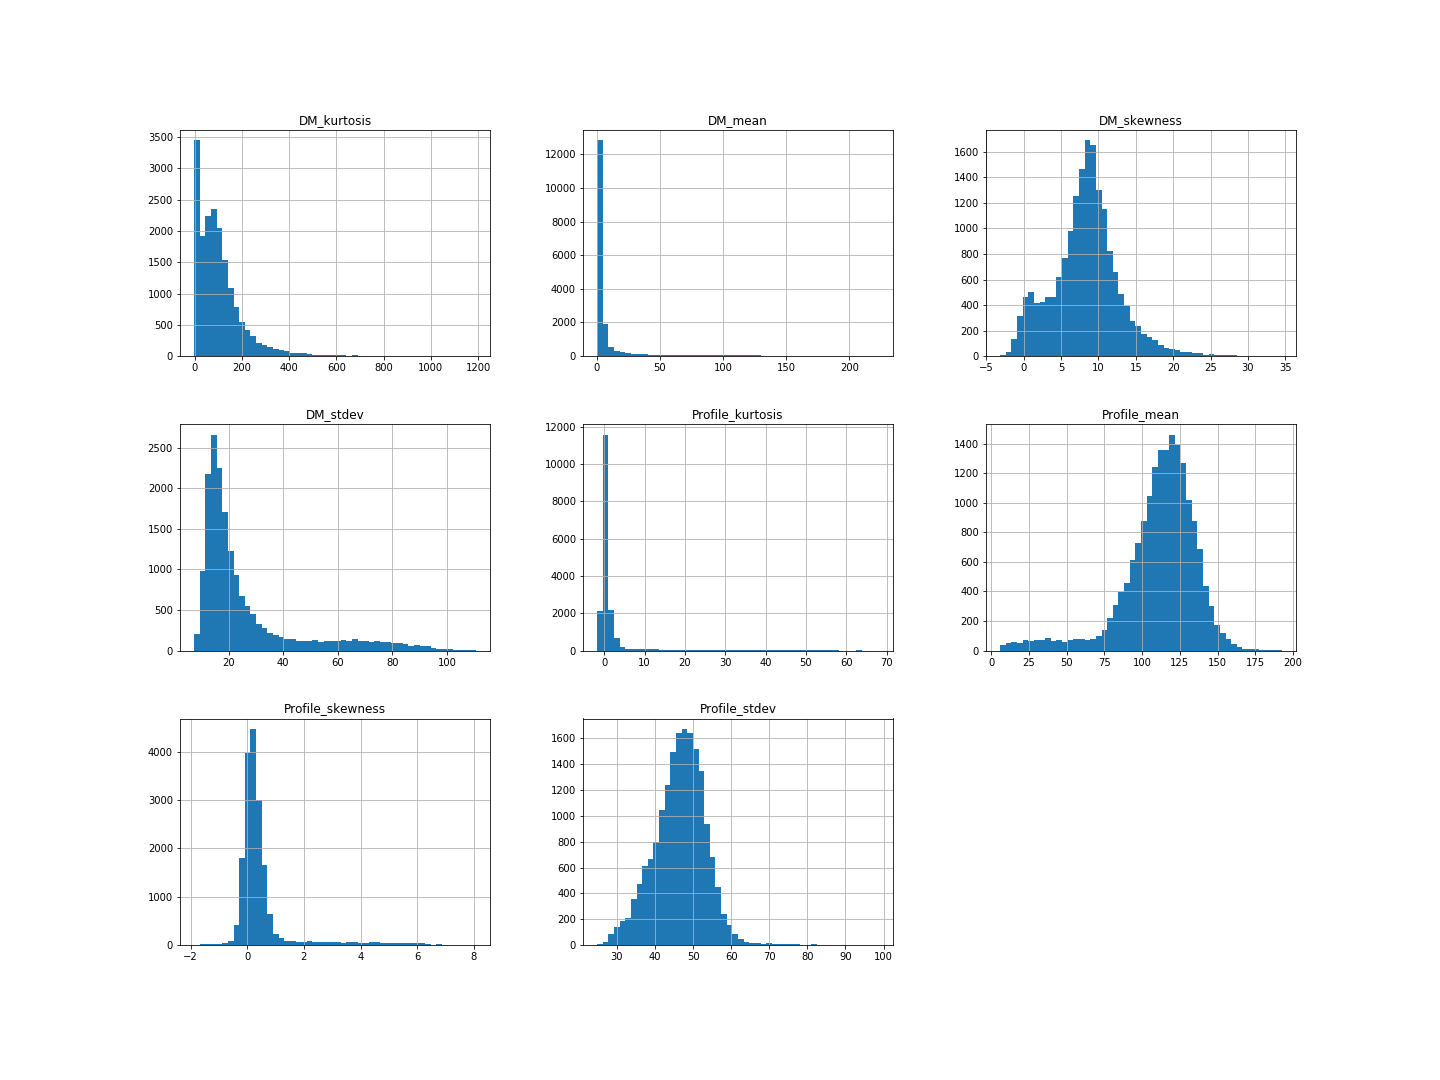
\includegraphics[scale=0.3]{img/distribution.png}
    \caption{Distribuições relativas às 8 variáveis contínuas. Por ordem, da esquerda para a direita, e de cima para baixo, temos: Curtose da curva \textit{DM-SNR}, Média da curva \textit{DM-SNR}, Assimetria da curva \textit{DM-SNR}, Desvio Padrão da curva \textit{DM-SNR}, Curtose do \textit{folded profile}, Média do \textit{folded profile}, Assimetria do \textit{folded profile} e Desvio padrão do \textit{folded profile}.}
    \label{fig:distribuicoes}
    \end{figure}
    
    Assim sendo, para esta tarefa de classificação binária os valores das oito variáveis relativas ao sinal são usados na análise de cada candidato, de forma a determinar se se trata ou não de um pulsar (informação fornecida na 9ª coluna do \textit{dataset}).
    
    \begin{figure}[t]
	\centering
	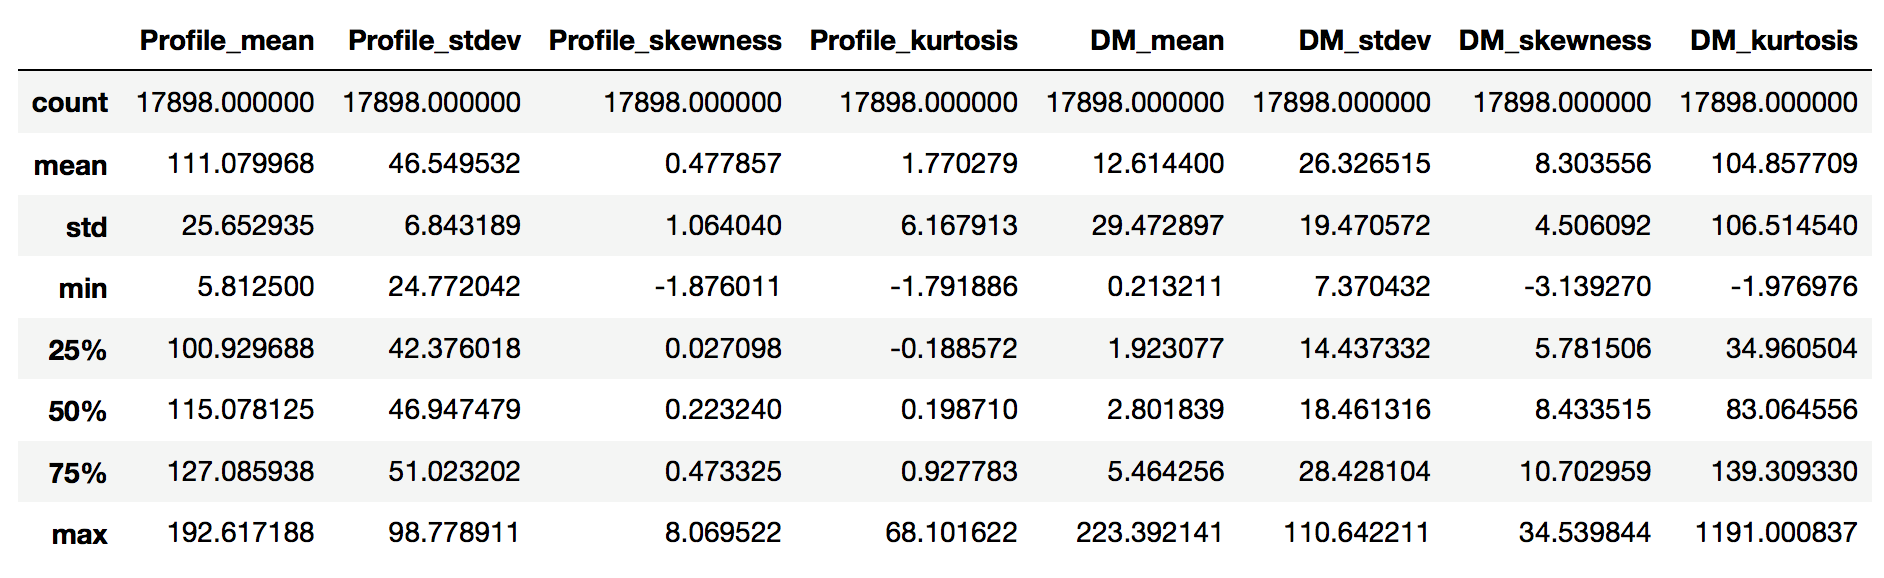
\includegraphics[scale=0.24]{img/distTable.png}
    \caption{Estatísticas descritivas sumárias, relativas às 8 variáveis de \textit{input}.}
    \label{fig:descricao_do_dataset}
    \end{figure}
    
%    \begin{center}
% 	\begin{tabular}{|c c c c c c c c c|} 
% 	\hline
% 	 & \textbf{FP\_mean} & \textbf{FP\_stdev} & \textbf{FP\_skewness} & \textbf{FP\_kurtosis} & \textbf{DM\_mean} & \textbf{DM\_stdev} & \textbf{DM\_skewness} & \textbf{DM\_kurtosis}\\ [0.5ex] 
% 	\hline\hline
% 	\textbf{count} & 17896.000000 & 17898.00000 & 787 \\ 
% 	\hline
% 	2 & 7 & 78 & 5415 \\
% 	\hline
% 	3 & 545 & 778 & 7507 \\
% 	\hline
% 	4 & 545 & 18744 & 7560 \\
% 	\hline
% 	5 & 88 & 788 & 6344 \\ [1ex] 
% 	\hline
%	\end{tabular}
%	\end{center}

\subsubsection{Pré-processamento dos dados.}
	Nesta secção, é descrito qual o pré-processamento aplicado ao conjunto de dados, explicando também as vantagens que daí advém.

	Relativamente à etapa de pré-processamento dos dados, temos duas considerações importantes: por um lado, todas as colunas de \textit{input} contêm valores de vírgula flutuante, de distribuição contínua; por outro lado, a coluna de \textit{output}, corresponde a uma de duas classes (classe positiva ou negativa, caso seja ou não um pulsar).
    
    Assim, para facilitar a aprendizagem por parte do algoritmo e contribuir para convergir mais rapidamente, fazemos normalização dos dados de input (\textit{feature scaling}), para uma escala no alcance [-1,1]. Por sua vez, relativamente à classe de \textit{output}, extraímos os dados para uma matriz unidimensional em que cada elemento tem um valor binário: 1 caso seja referente a um pulsar, e 0 em caso contrário.

\subsubsection{Modelo de aprendizagem a aplicar: redes neuronais.}
	Neste trabalho iremos usar uma rede neuronal artificial, \textit{Multilayer Perceptron} (MLP), que segue uma técnica de \textit{aprendizagem supervisionada} denominada \textit{backpropagation}. Assim, torna-se importante esclarecer cada um destes conceitos.

    Algoritmos que seguem o modelo da aprendizagem supervisionada são algoritmos nos quais os possíveis \textit{outputs} do algoritmo já são conhecidos e nos quais os dados usados para treinar o algoritmo já se encontram mapeados à resposta correta. Pode-se verificar que este modelo é aplicável ao problema dos pulsares na medida em que a totalidade das entradas na base de dados se encontram mapeados a um resultado, como na Secção~\ref{sec:dataset}.
    
    Por sua vez, \textit{backpropagation} é um método usado para o cálculo do gradiente de funções que regem as redes neuronais, sendo frequentemente usado no algoritmo de \textit{gradient descent}. Este é um algoritmo iterativo de otimização de primeira ordem, que permite encontrar o mínimo local de uma função.
    
	Dada uma rede neuronal artificial e uma função de erro (ou função de perda), o algoritmo de \textit{backpropagation}, também conhecido por algoritmo da propagação de erros para trás (\textit{backward propagation of errors}), calcula o gradiente da função de erro considerando sempre o peso das arestas na rede neuronal. Este cálculo é propagado para trás na rede neuronal, com o gradiente da última camada de pesos a ser calculado primeiro e o gradiente da primeira camada de pesos em último lugar (daí o seu nome \textit{backpropagation}). Este fluxo invertido da informação de erro permite uma computação eficiente do gradiente em cada camada, ao invés da abordagem ingénua de calcular o gradiente de cada camada separadamente.
    
    O algoritmo desenvolve-se em duas fases. Numa primeira fase, propaga-se através da rede de forma a chegar aos valores \textit{output}. De seguida, calcula o custo da propagação para cada output, sendo que esta estará intrinsecamente relacionada com a função de erro usada no algoritmo do gradiente descendente. Por fim, propaga-se em sentido contrário de forma a gerar um valor de erro para cada um dos neurónios. Na segunda fase, os pesos das arestas são constantemente atualizados conforme o resultado desempenhado por cada um dos candidatos. Na atualização das arestas é usado uma percentagem previamente definida como fator de atualização dos pesos. Quanto mais elevado for este fator, mais rápido será o treino da rede neural. Por outro lado, quanto mais baixo for este fator, mais preciso será o treino.
    
% Durante o desenvolvimento deste projeto, foram implementados dois modelos de aprendizagem: um primeiro em que as três camadas eram do tipo \textit{Convolutional}, \textit{Dense} e \textit{Dense}
    
\subsubsection{Arquitetura das redes neuronais.}
	As redes neuronais, surgiram com base na perceção biológica das interligações presentes no cérebro humano. Assim, tal como o cérebro humano é constituído por neurónios, os quais recebem impulsos nervosos como entrada e saída de dados, também as redes neuronais são constituídas por camadas de neurónios, ativados com estímulos específicos. Um neurónio tem a capacidade de estimular os seus neurónios vizinhos, quando este é propriamente estimulado (função de ativação). Posto isto, podemos definir matematicamente um neurónio como sendo:
    \begin{figure}[H]
    \centering
    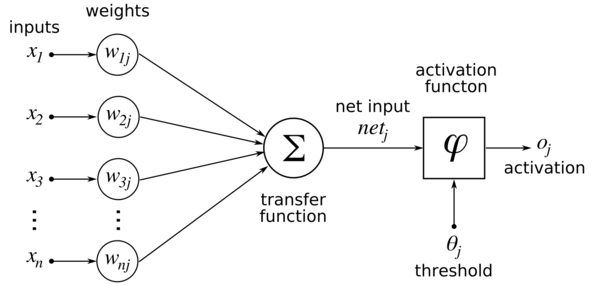
\includegraphics[scale=.5]{img/neural.png}
    \caption{Modelo natemático de um neurónio.}
    
    \LARGE{\[ y = f_\textit{ativação} (\sum_{i} w_ix_i - \theta ) \]}
    \caption{Representação matemática da saída de um neurónio.}
    \end{figure}
    
    Como o nome indica, é uma rede, por isso a sua consistência detêm vários neurónios conectados na forma de um grafo acíclico. As redes neuronais mais comuns, \textit{feedforward}, são redes em que o \textit{output} de certos neurónios é o \textit{input} de outros.
Desta forma é possível separar a rede em diferentes camadas:
	\begin{enumerate}
		\item Uma \textbf{\textit{Input Layer}}, primeira camada na rede neuronal, responsável por receber os dados, determinar o tamanho do \textit{dataset} e apresentar os padrões de reconhecimento. São apenas constituídas por neurónios de \textit{input}.
		\item Uma ou mais \textbf{\textit{Hidden Layer}}, é nesta(s) camada(s) que é feita maior parte da aprendizagem dos pesos do modelo. Camadas seguidas deverão corresponder a \textit{features} cada vez mais abstratas, permitindo alcançar um modelo generalizável e de bom desempenho.
        \item Uma \textbf{\textit{Output Layer}}, última camada da rede, responsável por apresentar os dados, esta camada é constituída com um número de neurónios geralmente igual ao número de classes de \textit{output} (ou apenas 1 se se tratar de classificação binária). É uma camada que não dispõe de função de ativação, e os cujos são exclusivamente neurónios de \textit{output}.
	\end{enumerate}
    
    \begin{figure}[H]
    \centering
    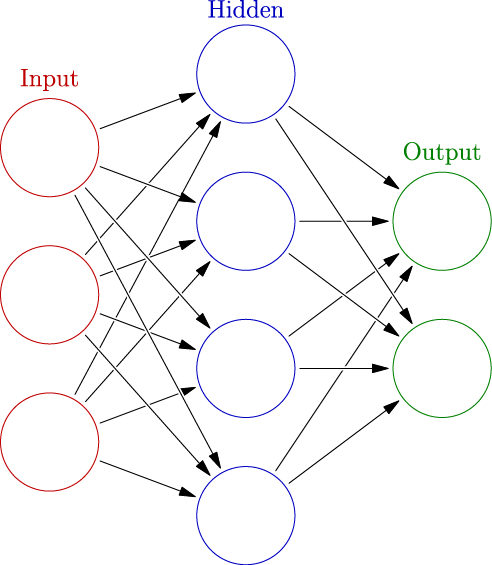
\includegraphics[scale=.7]{img/neural_network.png}
    \caption{Representação Abstrata da Rede Neural}
    \end{figure}
    
\subsubsection{Configuração da rede neuronal.}
    Partindo agora para o nosso caso em concreto, é sempre muito complicado prever a configuração/arquitetura da rede ideal para um dado problema, isto é, qual o número ideal de \textit{hidden layers}, qual o número de neurónios das camadas, qual o tipo de funções de ativação usadas, entre outras variações. Por isso é algo que requer alguns testes com diferentes composições para se obter os melhores resultados, coadjuvados por métodos de \textit{Grid Search}, testando um conjunto de combinações promissoras e melhorando iterativamente.
    
    Neste sentido, foram desenvolvidos testes ao número de \textit{hidden layers}, variando entre 1 a 2 o número destas \textit{layers}, e variando também o número de neurónios em cada uma entre 8, 12, 16, ou 32. Como função de ativação, foi usada a função ``relu'' para as camadas intermédias (\textit{hidden}).
    A camada de \textit{input} terá obrigatoriamente 8 entradas (uma por variável), e a camada de \textit{output} tem apenas 1 neurónio, ativado pela função ``sigmoid'', de modo a balisar o \textit{output} entre 0 e 1 (indicativo do grau de certeza de o candidato se tratar ou não de um pulsar).
    Os resultados destas configurações são apresentados na Secção~\ref{sec:trabalho}.

\subsubsection{Forma de Avaliação}
\label{sec:avaliacao}
Para nos assegurarmos que o modelo cumpre os requisitos, iremos dividir o \textit{dataset} em duas partes, com 80\% e 20\%, usando a primeira para treino do modelo, e a segunda para avaliação do seu desempenho.

Assim, e tendo em conta a tarefa em questão, será muito útil ter em atenção o \textit{recall} da classe positiva, pois queremos maximizar a identificação de pulsares. Neste sentido, as métricas usadas para avaliação dos modelos serão a precisão global do modelo (\textit{accuracy}), o \textit{recall} da classe positiva, bem como o \textit{F1 score}. O \textit{F1 score} consiste numa média harmónica da precisão e do \textit{recall} para cada uma das classes em causa.

Adicionalmente, todos os testes terão que ter validação cruzada em \textit{k} partes (\textit{k-fold cross-validation}), de modo a diminuir os efeitos da aleatoriedade no treino dos modelos.

\subsection{Trabalho Efetuado}
\label{sec:trabalho}
Como referido na secção anterior, foram realizados vários testes, com diferentes configurações da rede neuronal. Os resultados, medidos no \textit{dataset} de teste, estão apresentados na Tabela~\ref{tab:resultados}. Como podemos ver, atingimos resultados muito promissores, sendo que o melhor modelo tem duas \textit{hidden layers}, com 32 e 16 neurónios. Todos os testes foram realizados com \textit{3-fold cross-validation}, sendo facilmente reproduzíveis.

Para a realização/codificação dos modelos de redes neuronais, bem como para a sua avaliação, foi usada a linguagem de programação \textit{Python}, bem como as \textit{frameworks} Keras, Tensorflow e Scikit-learn. Para o tratamento e visualização de dados foram usadas as \textit{frameworks} \textit{NumPy}, \textit{Pandas} e \textit{MatPlotLib}.

\begin{table}[t!]
\centering
  \begin{tabular}{lll}
  \hline
  First Hidden Layer & Second Hidden Layer & Accuracy \\ \hline
  32                 & 32                  & 98.02    \\
  32                 & 16                  & 98.07    \\
  32                 & 12                  & 98.16    \\
  32                 & 8                   & 98.01    \\
  16                 & 12                  & 97.93    \\
  16                 & 8                   & 97.74    \\
  8                  & 8                   & 97.76    \\
  32                 & -                   & 96.41    \\
  16                 & -                   & 96.08    \\ \hline \\
  \end{tabular}
  \caption{Resultados obtidos com diferentes configurações da rede neuronal.}
  \label{tab:resultados}
\end{table}

\subsection{Trabalho Futuro}
Apesar de termos atingido resultados muito promissores, falta ainda uma avaliação mais profunda aos modelos gerados, particularmente avaliando o \textit{F1 score} de cada um, como referido na Secção~\ref{sec:avaliacao}.

Para além disso, achamos possível melhorar estes resultados com algumas variações na configuração da rede, nomeadamente:
\begin{itemize}
  \item Uso de camadas Convolucionais unidimensionais;
  \item Uso de regularização L1 e/ou L2;
  \item Experimentação com diferentes funções de ativação;
  \item Realização de \textbf{\textit{undersampling}}, visto os exemplos da classe negativa serem 10 vezes mais comuns que os da classe positiva, retirando alguns dos exemplos negativos do \textit{dataset} de treino.
\end{itemize}


%************************************************************************************
%************************************************************************************

\section{Conclusões}
	Primeiramente, acreditamos que o nosso conhecimento sobre redes neuronais foi consideravelmente aprofundado, mostrando-se assim o grupo satisfeito com a escolha de tema realizada. De facto, Redes Neuronais artificiais representam um abordagem a problemas bastante atual, contribuindo assim ainda mais para o interesse do grupo no trabalho.   
    
    É também evidente que Redes Neuronais artificiais se revelam uma ferramenta extremamente útil, apropriada para resolver problemas semelhantes ao apresentado, resultando numa abordagem ao problema bastante diferente de tudo aquilo com o que nós, como alunos do 3º ano de Informática, tínhamos tido a oportunidade de trabalhar.
    
    Em suma, os resultados obtidos revelaram-se promissores, sendo a precisão do melhor modelo apresentado superior a 98\%. Ainda assim, o grupo considera ser possível melhorar o desempenho da rede neuronal artificial implementada, através da experimentação com diferentes camadas e configurações.
    
\newpage

%************************************************************************************
%************************************************************************************

\section{Recursos}

Abadi, Martín, Paul Barham, Jianmin Chen, Zhifeng Chen, Andy Davis, Jeffrey Dean, Matthieu Devin et al. "TensorFlow: A System for Large-Scale Machine Learning." In OSDI, vol. 16, pp. 265-283. 2016.
\\

Chollet, François. "Keras." KerasCN Documentation (2017): 55.
\\

Pedregosa, Fabian, Gaël Varoquaux, Alexandre Gramfort, Vincent Michel, Bertrand Thirion, Olivier Grisel, Mathieu Blondel et al. "Scikit-learn: Machine learning in Python." Journal of machine learning research 12, no. Oct (2011): 2825-2830.
Harvard	
\\

Lyon, Robert James. "Why are pulsars hard to find?." PhD diss., University of Manchester, 2016.
\\

R. J. Lyon, B. W. Stappers, S. Cooper, J. M. Brooke, J. D. Knowles, Fifty Years of Pulsar Candidate Selection: From simple filters to a new principled real-time classification approach, Monthly Notices of the Royal Astronomical Society 459 (1), 1104-1123, DOI: 10.1093/mnras/stw656
\\

Ruck, Dennis W., Steven K. Rogers, Matthew Kabrisky, Mark E. Oxley, and Bruce W. Suter. "The multilayer perceptron as an approximation to a Bayes optimal discriminant function." IEEE Transactions on Neural Networks 1, no. 4 (1990): 296-298.
\\


\newpage

\end{document}